\documentclass{report}

\author{Nikhil Verma}
\usepackage{tikz}
\usepackage{amsfonts}
\usepackage{geometry}
\geometry{
    a3paper
}
\usetikzlibrary{trees}


% See https://tikz.dev/tikz-trees
% See https://latexdraw.com/draw-trees-in-tikz/

\begin{document}

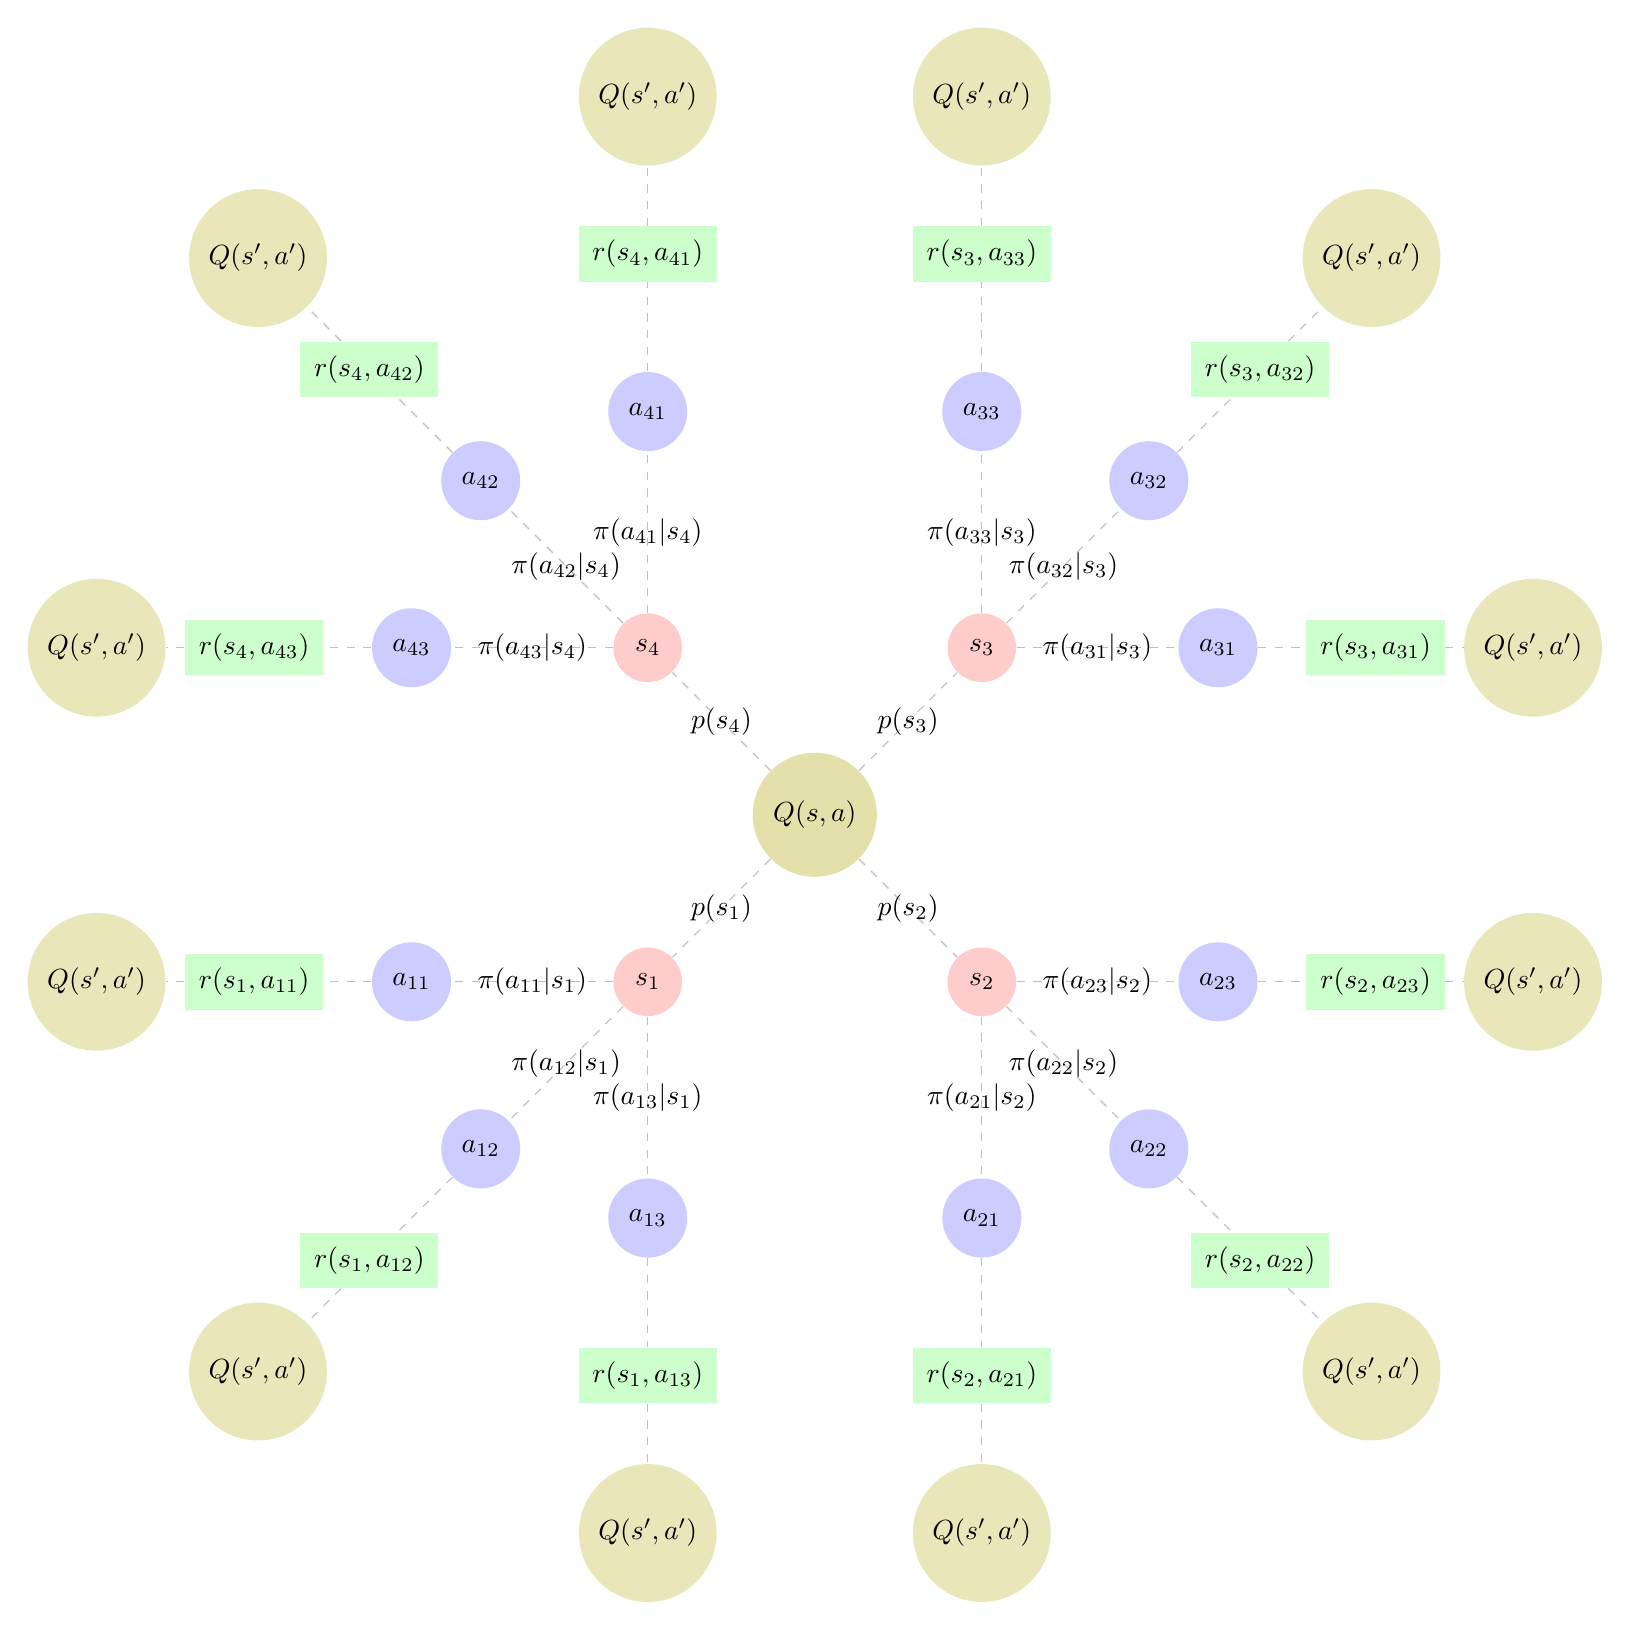
\begin{tikzpicture}
	[
        grow cyclic,
        % styles
        prob/.style = {opacity = 1},
        state/.style = {circle, fill = red!20},
        action/.style = {circle, fill = blue!20},
        reward/.style = {rectangle, fill = green!20},
        exp/.style = {circle, fill = olive!20},
        % defaults
        edge from parent/.style = {draw, dashed, opacity = 0.25},
        every node/.style = {opacity = 1, inner sep = 5pt},
        % levels
		level 1/.style = {sibling angle = 90, level distance = 3cm},
		level 2/.style = {sibling angle = 45, level distance = 3cm},
		level 3/.style = {sibling angle = 30, level distance = 20mm},
		% edge from parent path = {(\tikzparentnode\tikzparentanchor) .. controls +(0,-1) and +(0,1) .. (\tikzchildnode\tikzchildanchor)}
	]
	\coordinate node [circle, inner sep = 5pt, fill = olive!25] {$Q(s, a)$}
	child foreach \x in {1,2,3,4} {
        node [state] {$s_\x$} {
            child foreach \y in {1,2,3} {
                node [action] {$a_{\x\y}$} {
                    child {
                        node [reward] {$r(s_\x, a_{\x\y})$}
                            child {node [exp] {$Q(s', a')$}}
                    }
                }
            edge from parent node [prob] {$\pi(a_{\x\y}|s_\x)$}
            }
        }
        edge from parent node [prob] {$p(s_\x)$}
    };
\end{tikzpicture}

\end{document}